\section{$(t, x, z)$空间内的有限差分}
\label{sec:2.7}

如果不是大多数,至少也是很多生产性的偏移处理工作都是在$(t,x,z)$空间内完
成的。为避免被这种三维空间的复杂性所纠缠,我们将首先考虑一下固定$k_x$时在$(z,t)$二
维空间内的偏移。

\subsection{$(z,t)$空间内的偏移}
\label{sec:2.7.1}

可以在$(z',t')$空间内按下列包含有上行波$U$的表格来考察偏移与数据合成的处理过程。
\begin{figure}[H]
\centering
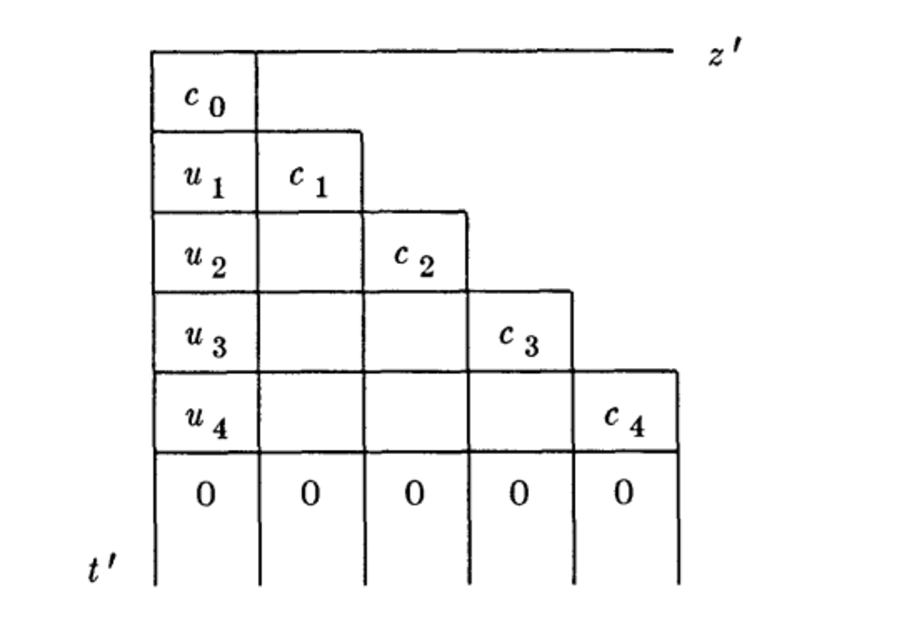
\includegraphics[width=0.65\textwidth]{new/fig-2-7-1}
\caption{差分表}
\label{fig:new/fig-2-7-1}
\end{figure}
在这个表中,在地面$z'=0$所观测到的上行波以$u_t$表示;以$c_t$表示的偏移剖而则沿对角线显
示,因为时间$t=0$时的爆炸反射面的成像条件是在延迟空间内用下式表示的
\begin{subequations}
\begin{equation}
z'=z
\label{eq:ex2.7.2a}
\end{equation}
\begin{equation}
t'=t+z/v
\label{eq:ex2.7.2b}
\end{equation}
\label{eq:ex2.7.2}
\end{subequations}
\begin{equation}
0=t=t'-z'/v
\label{eq:ex2.7.3}
\end{equation}
有最佳聚焦作用的偏移结果并不需要全落在表中所示的45°线上,它可以位于任何直线
上或曲线上,这主要决定于地层的速度。这种曲线构成了速度测定方法的基础(见\ref{sec:3.5}
节), 而在频率域内你就不可能按这种方式来确定速度。

根据\ref{sec:2.1}节的结论,延迟坐标$(t',x',z')$内的上行波$U$的方程为
\begin{equation}
\frac{\partial^2 U}{\partial z'\partial t'}=-\frac{v}{2}\frac{\partial^2 U}{\partial (x')^2}
\label{eq:ex2.7.4}
\end{equation}
然后,对$x$轴迸行Fourier变换,这要假设$v$是$x$的恒定函数,而且假设$U$对$x$的依从关系是正
弦塑函数$\exp(ik_xx)$,因而
\begin{equation}
0=(\frac{v}{2}k_x^2-\frac{\partial^2 }{\partial z'\partial t'})U
\label{eq:ex2.7.5}
\end{equation}
现在,要把这个偏微分方程按广与进行离散化,将要采用矩阵符号,不过'并不是属
于矩阵代数的符号,而是指置于\ref{fig:new/fig-2-7-1}所示表之$(t',z')$平面上的差分系数组成的矩
阵。令符号$*$来代表$(z,t)$空间内的褶积运算,相继求导数实际是一种褶积过程,所以
$\partial/\partial z \partial/\partial t=\partial^2/(\partial z\partial t)$这种概念用下式表示:
\begin{equation}
\begin{bmatrix}
-1 & +1
\end{bmatrix}
*
\begin{bmatrix}
-1 \\
1
\end{bmatrix}
=
\begin{bmatrix}
1&-1\\
-1&1
\end{bmatrix}
\label{eq:ex2.7.6}
\end{equation}
所以,式\ref{eq:ex2.7.5}的差分形式为
\begin{equation}
0=\{\frac{v}{2}\frac{\Delta z'\Delta t'}{4}k_x^2
\begin{bmatrix}
1&1\\
1&1
\end{bmatrix}
-
\begin{bmatrix}
1&-1\\
-1&1
\end{bmatrix} 
\}*U
\label{eq:ex2.7.7}
\end{equation}
其中出现$1/4$是因为要在网格的四个位置上取$U$的平均。

两个算子之和按下列形式恒有$\mid b \mid \geq \mid s \mid $
\begin{equation}
0 = 
\begin{bmatrix}
s&b\\
b&s
\end{bmatrix}
*U
\label{eq:ex2.7.8}
\end{equation}
现在将利用式\ref{eq:ex2.7.8}中的差分系数以各$U$值来填满\ref{fig:new/fig-2-7-1}所示的表。

已知三个方格中的$U$值,则可根据下面隐含的两种运算中的一种
\begin{figure}[H]
\centering
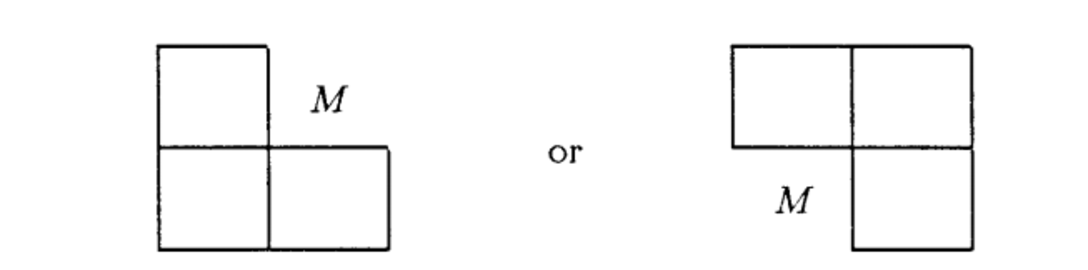
\includegraphics[width=0.65\textwidth]{new/fig-2-7-2}
\caption{左边a,右边b}
\label{fig:new/fig-2-7-2}
\end{figure}

就能够决定缺失的一个值$M$。可证明,由于$\mid b \mid \geq \mid s \mid $,按下面的格式进行$M$值的计算是不稳
定的:
\begin{figure}[H]
\centering
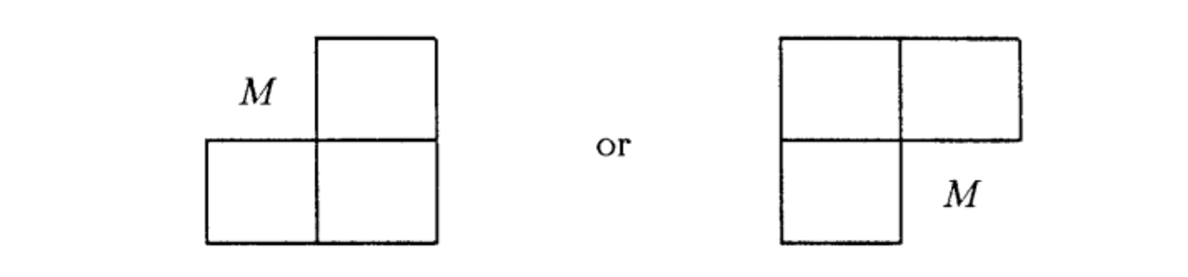
\includegraphics[width=0.65\textwidth]{new/fig-2-7-3}
\caption{左边a,右边b}
\label{fig:new/fig-2-7-3}
\end{figure}
很显然,如果$s$等于零,就会存在用零来除的问题。根据稳定性分析毫无困难就可证明,式
\ref{fig:new/fig-2-7-3}的运算方式会引起微小扰动呈指数增长。

有一个值得作一作的练习:在零倾角假设$(k_x=0)$下,用式\ref{eq:ex2.7.8}的算子中的数值
去填满\ref{fig:new/fig-2-7-1}所示表中的各元素.将会发现,$u_t$值沿$z$方向横向移动通过该表而无变化,
正如由该表所能预料到的,这意味着$c_t=u_t$。沿$z$方向有缓慢变化,就是提醒我们,沿$z$轴的
采样已经过密了。实际上,沿$z$轴迸行少量点的采样要比通常沿$t$轴进行采样节省很多计算时
间。

\subsection{$(t,x,z)$空间的15度绕射程序}
\label{sec:2.7.2}
